%%% Simulering af PWM-controller for 2. iteration

\subsection{PWM-controller}
I det følgende afsnit simuleres funktionaliteterne omkring PWM-controlleren. Her simuleres frekvensen af savtandspændingen og selve switch-frekvensen, samt signalet over current-sense modstanden både før og efter filteret.

\subsubsection{Switch-frekvens}
\noindent Først simuleres frekvensen af savtandspændingen. Dette er gjort på figur~\ref{fig:Simulering_PWM_savtand}. Periodetiden af savtandspændingen aflæses til $5.01\micro s$. Omregnet til en frekvens giver det: $f_{osc}=\frac{1}{5.01\micro s}=199.6k\hertz$. Derudover aflæses signalets minimumsspænding til ca. $138mV$, og maksimum- til ca. $2.5V$. I følge teorien burde spændingen ligge mellem $200mV$ og $2.65V$.

\begin{figure}[H]
	\center
	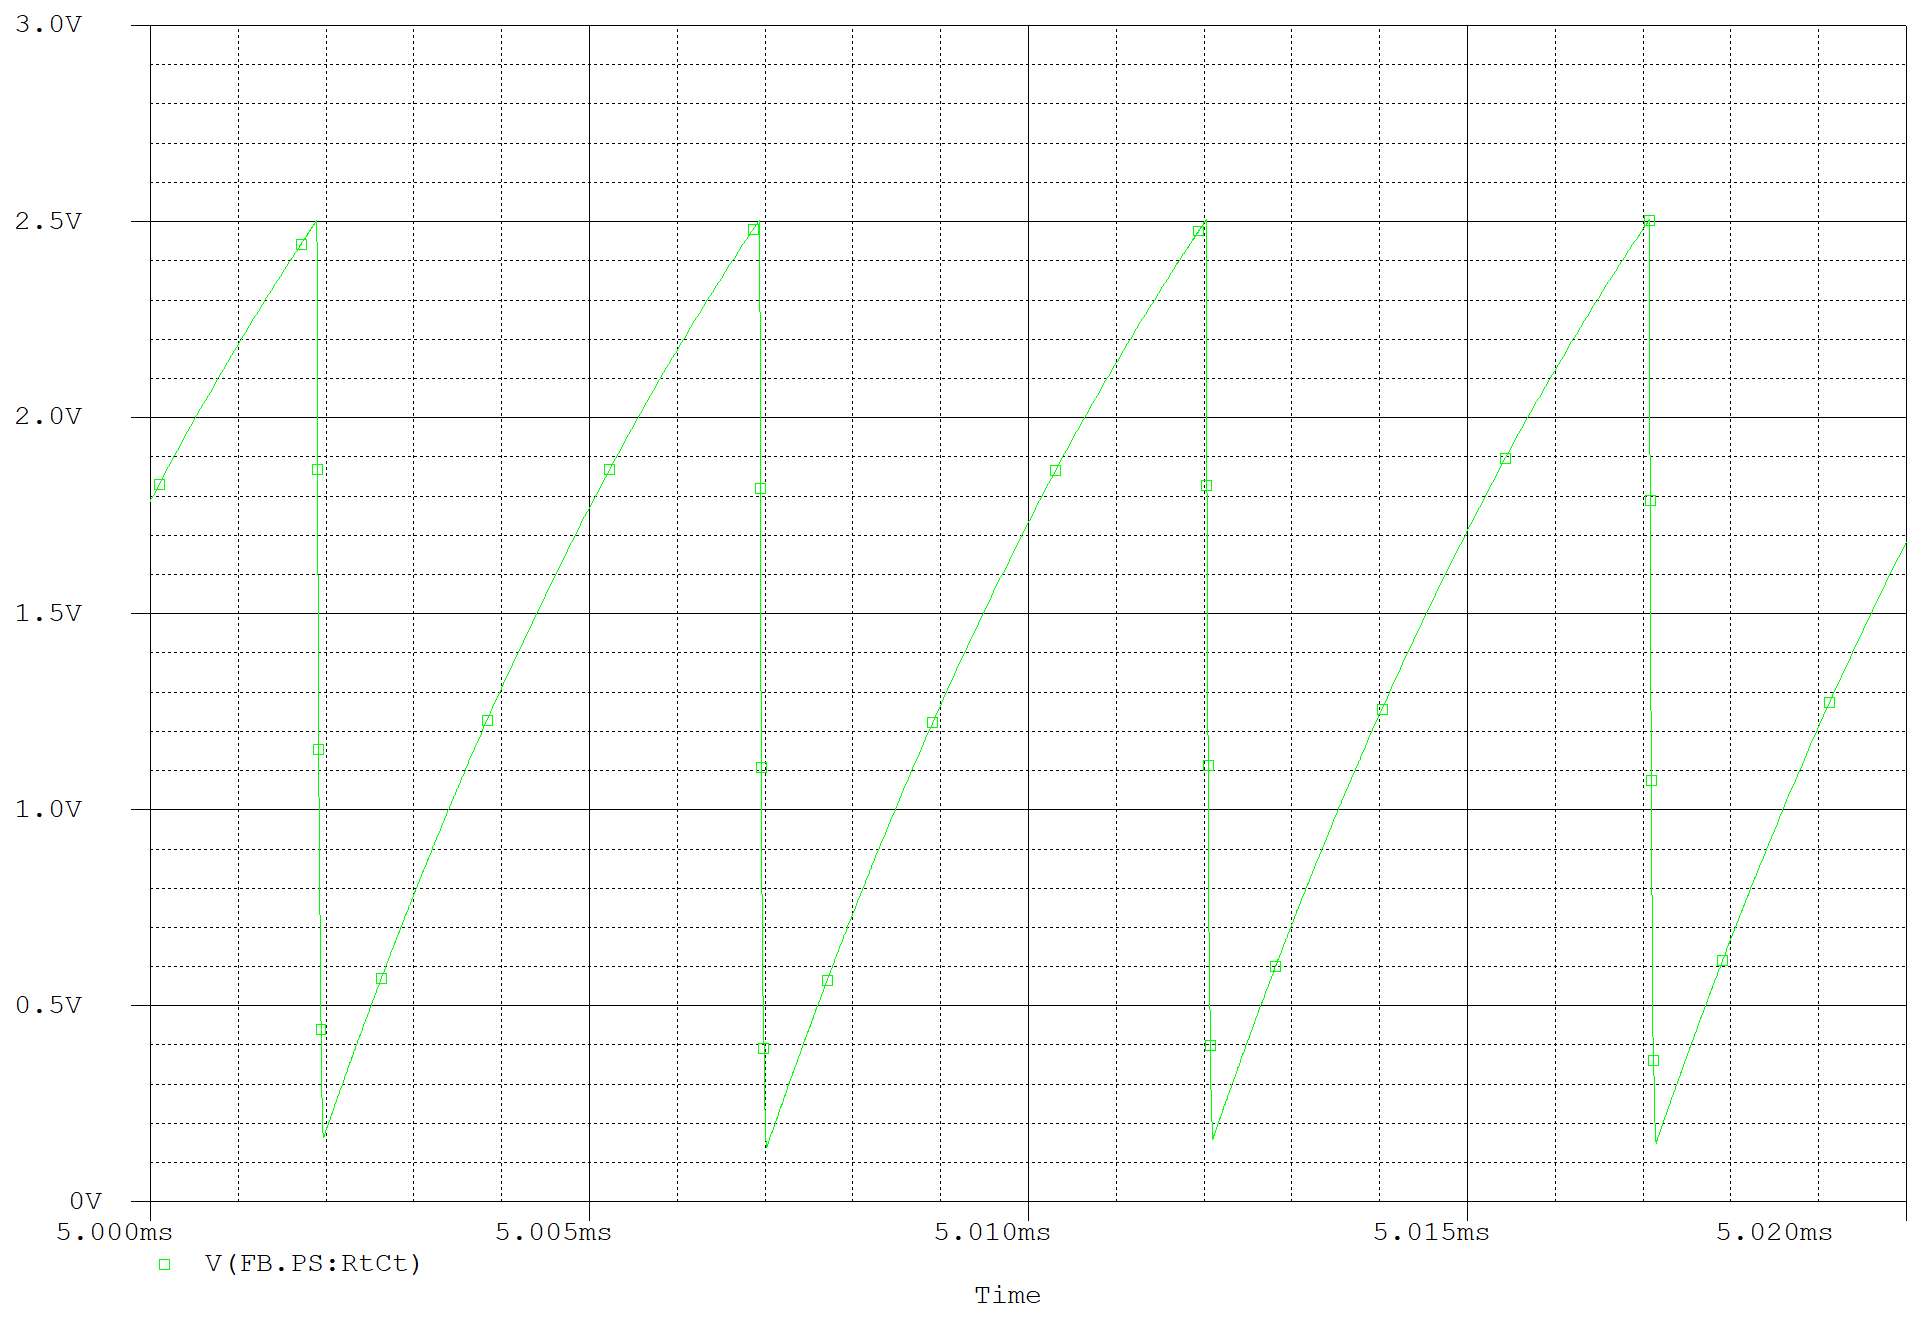
\includegraphics[max width=0.9\linewidth]{/tex/2iteration/billeder/Simulering_PWM_savtand.png}
	\caption{Simulering af savtandspændingen}
	\label{fig:Simulering_PWM_savtand}
\end{figure}

\noindent Nu simuleres selve switch-frekvensen. Dette er gjort på figur~\ref{fig:Simulering_PWM_switch_frekvens}, hvor der måles på udgangen af PWM-controlleren. Her måles periodetiden til $10.1\micro s$, eller en frekvens på $f_s=99.01k\hertz$. 

\begin{figure}[H]
	\center
	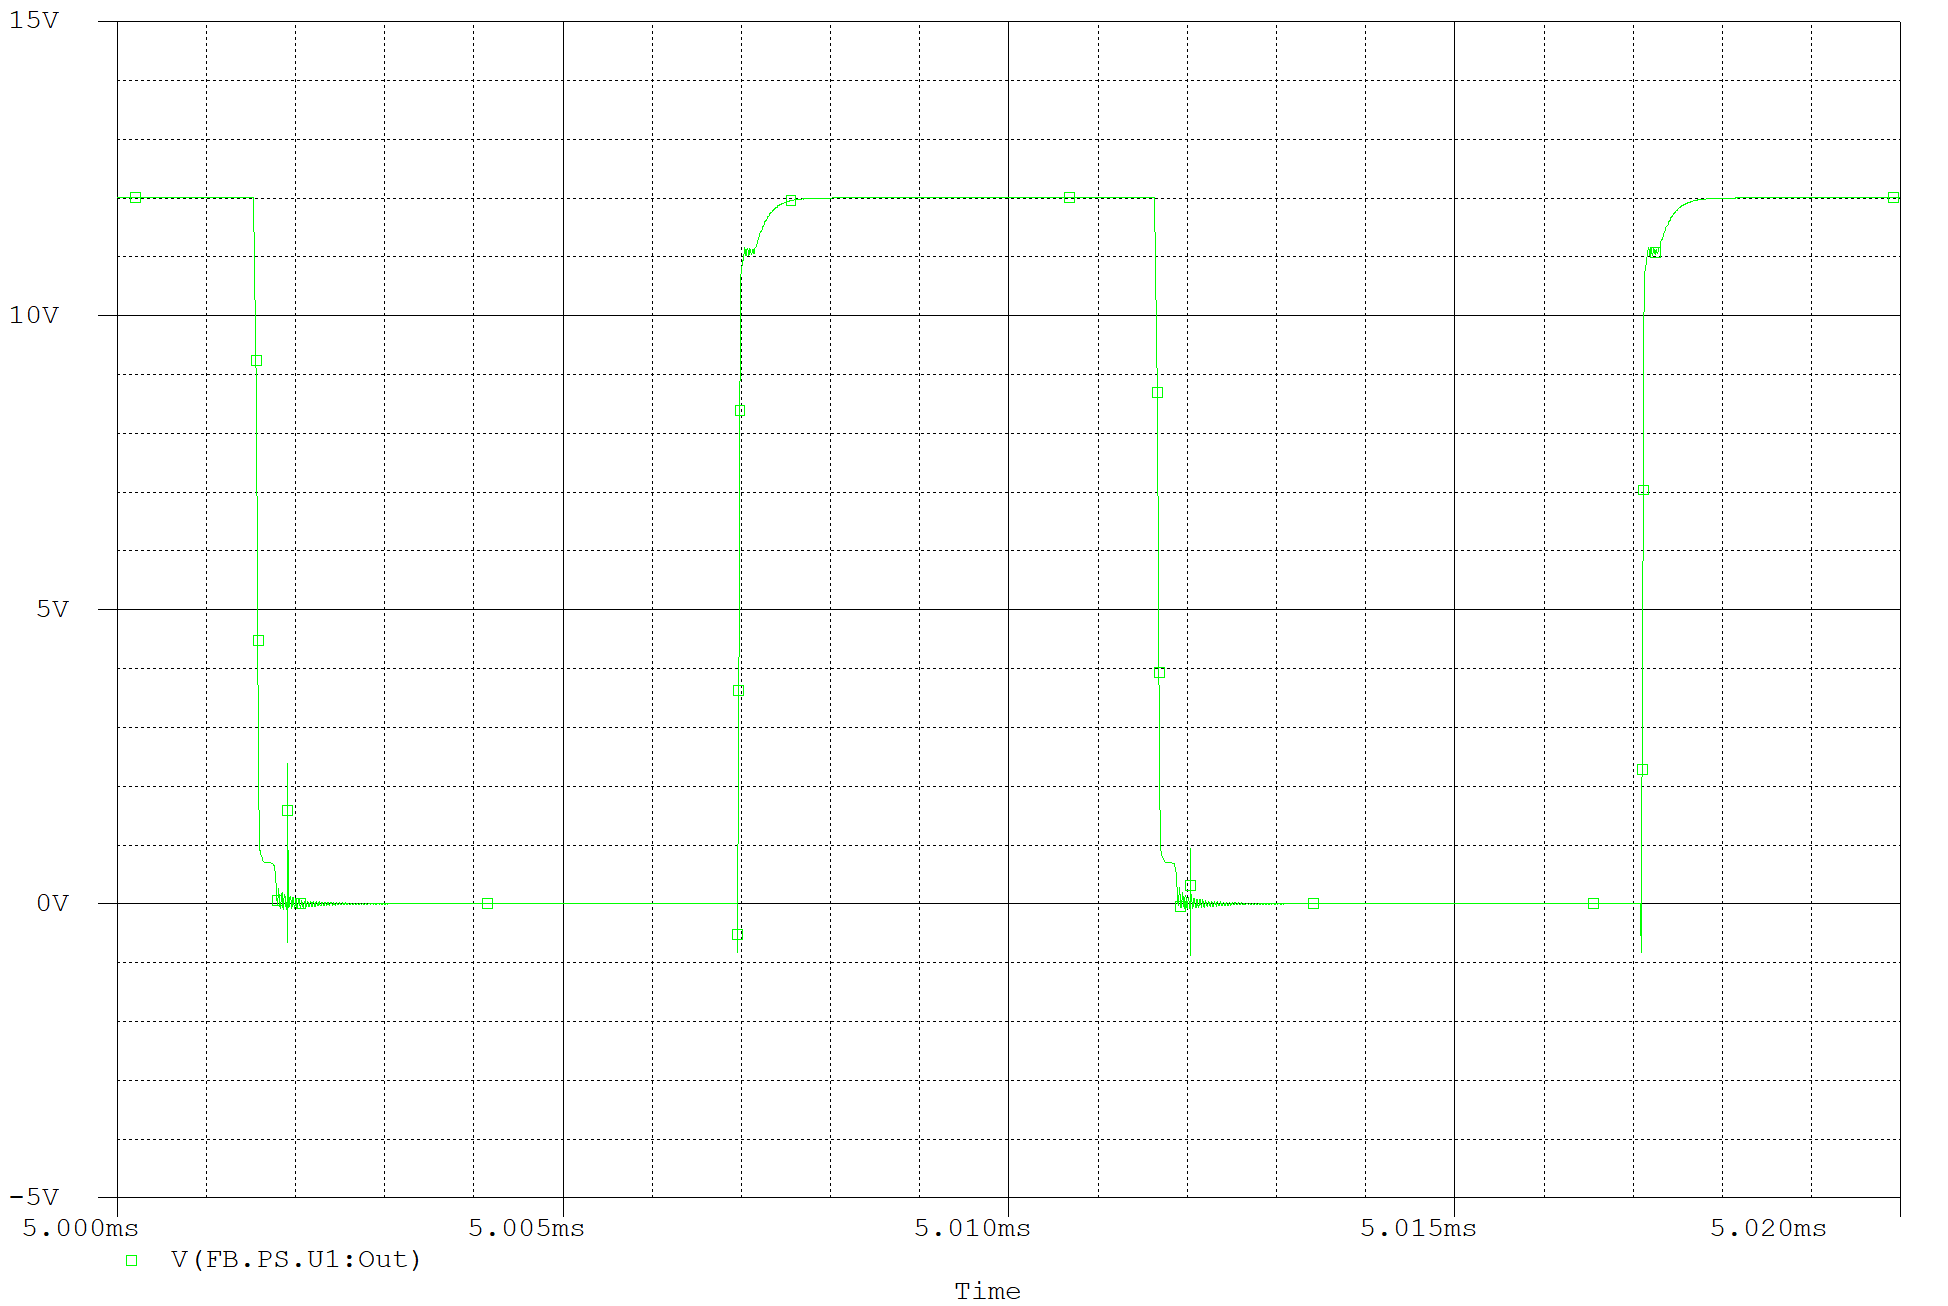
\includegraphics[max width=0.9\linewidth]{/tex/2iteration/billeder/Simulering_PWM_switch_frekvens.png}
	\caption{Simulering af switch-frekvens}
	\label{fig:Simulering_PWM_switch_frekvens}
\end{figure}

\subsubsection{Switch-tid}
\noindent Simuleringen af switch-tiden i MOSFET'en er vist på figur~\ref{fig:Simulering_MOSFET_switch_tid}. Figuren viser et zoom af MOSFET'ens gate signal. Switch-tiden kan aflæses som tiden af signalets plateau. Det aflæses til ca. $103ns$. Grunden til dette afviger meget fra analysen, er modellen for den MOSFET der bruges i simuleringen. Som nævnt bruges en anden MOSFET i simuleringen, end der er regnet med i analysen. En af de specifikationer de afviger mellem de to MOSFETs er \textit{Miller} ladningen, der bruges til at regne switch-tiden. I databladet for IRF630\cite{IRF630}, aflæses den til $15nC$. Regnes switch-tiden ud fra det, fås $107.1ns$, hvilket stemmer med det simulerede. 
\begin{equation} 
T_{ch} = \frac{Q_{gd} \cdot R_{g}}{V_{DD}-V_{gs}} = \frac{15nC \cdot 50\ohm}{12V-5V} = 107.1ns
\end{equation}

\begin{figure}[H]
	\center
	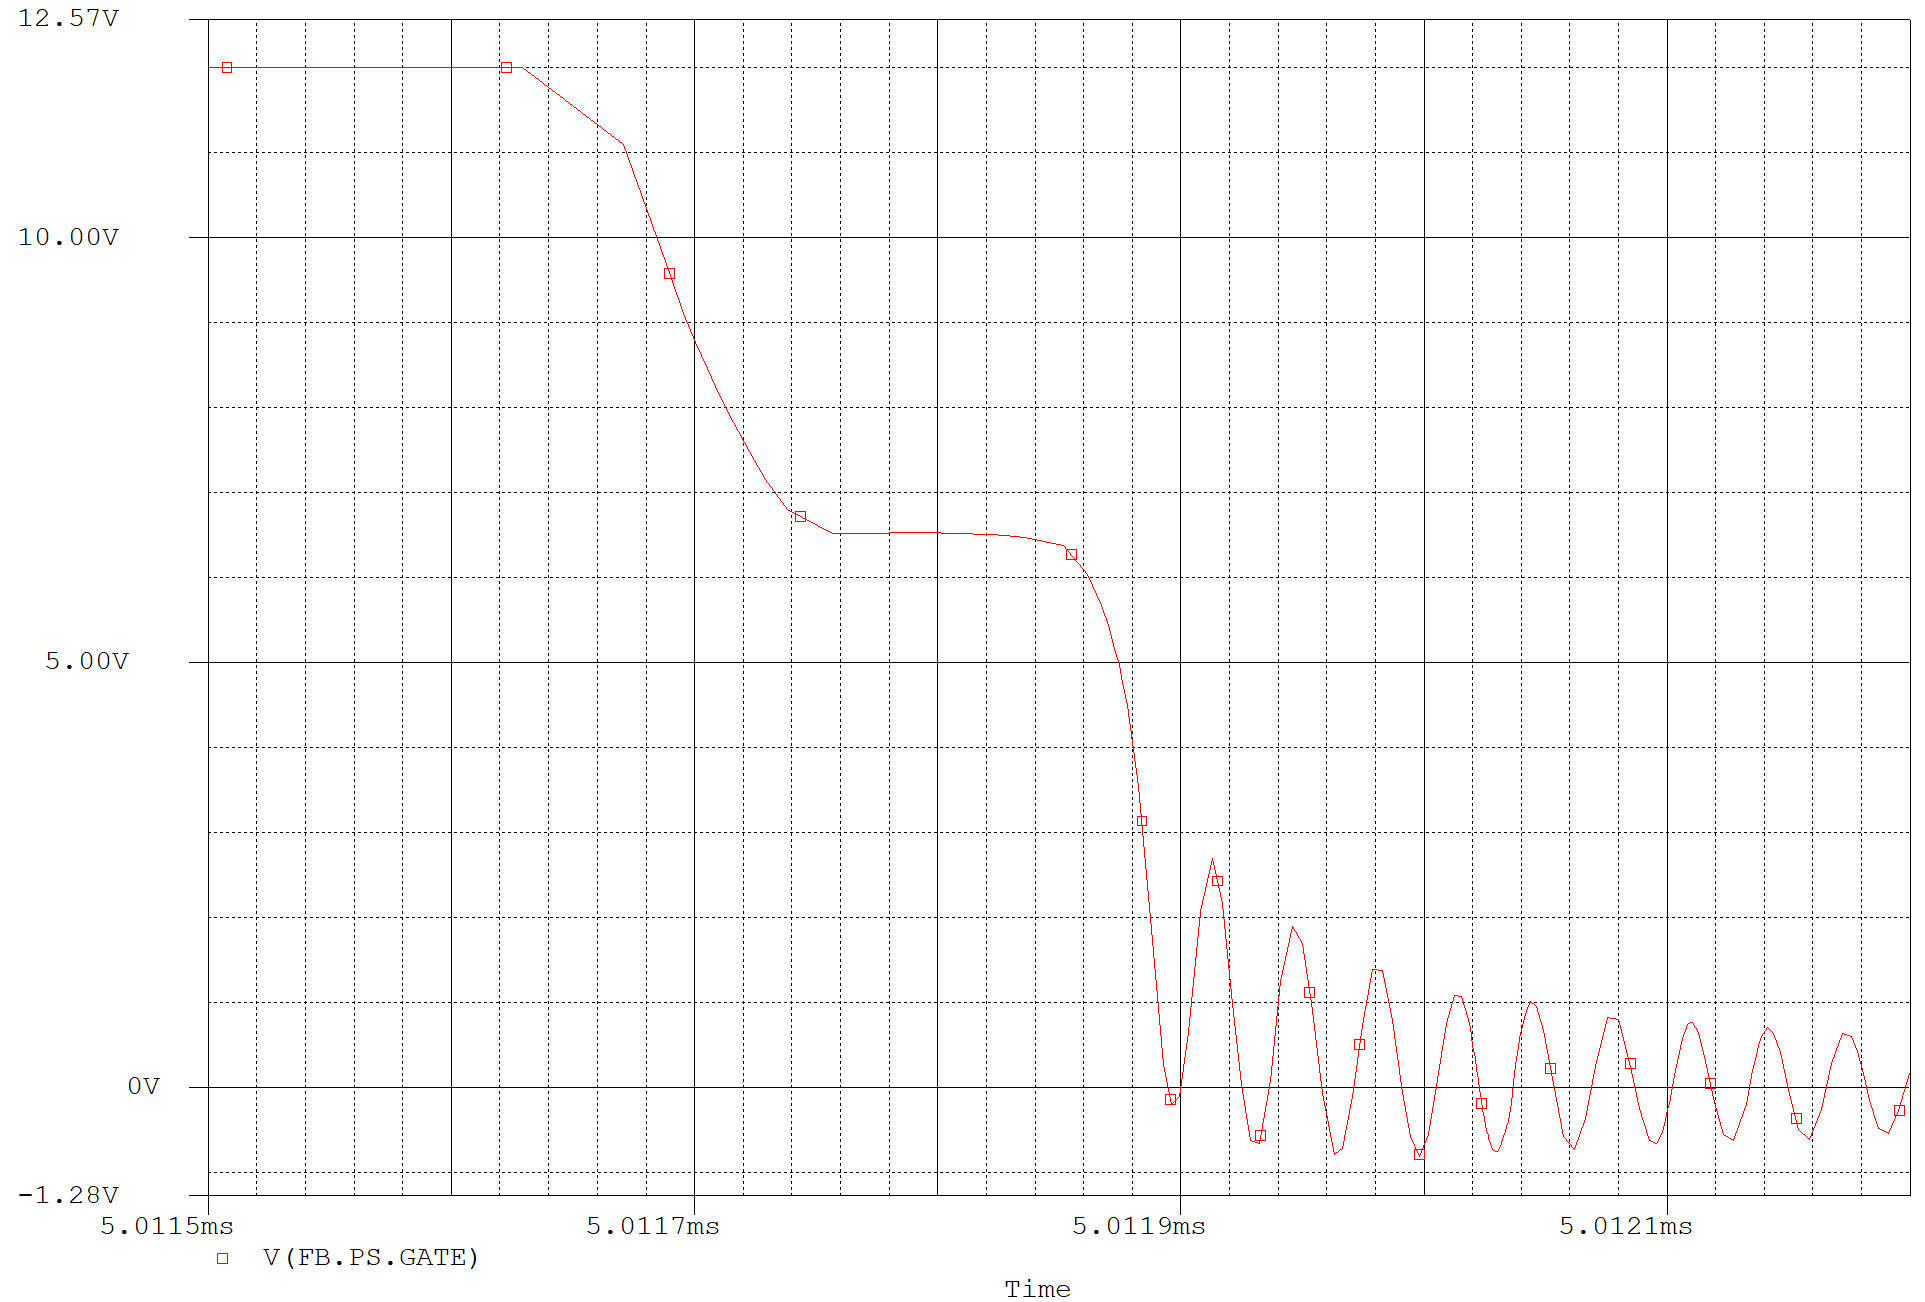
\includegraphics[max width=0.9\linewidth]{/tex/2iteration/billeder/Simulering_MOSFET_switch_tid.png}
	\caption{Simulering af switch-tid i MOSFET}
	\label{fig:Simulering_MOSFET_switch_tid}
\end{figure}


\subsubsection{Current-sense}
\noindent Current-sense signalet måles både før og efter filtreringen. Signalet før filteret ses på figur~\ref{fig:Simulering_PWM_current_sense_U}. Her ses de spikes på signalet, der kan give anledning til en forkert duty-cycle. Figur~\ref{fig:Simulering_PWM_current_sense_M} viser simuleringen for signalet efter filtreringen. Her ses det, at spikesene er blevet filtreret væk, dog med den konsekvens at signalet har fået en langsommere stigetid. Stigetiden aflæses til ca. $280ns$. Ifølge teorien burde PWM-controllerens udgangssignal skifte, når current-sense signalet er lig $1V$. På figur~\ref{fig:Simulering_PWM_current_sense_M}, ses det, at dette også er tilfældet for p-spice modellen for UCC1801. 


\begin{figure}[H]
	\center
	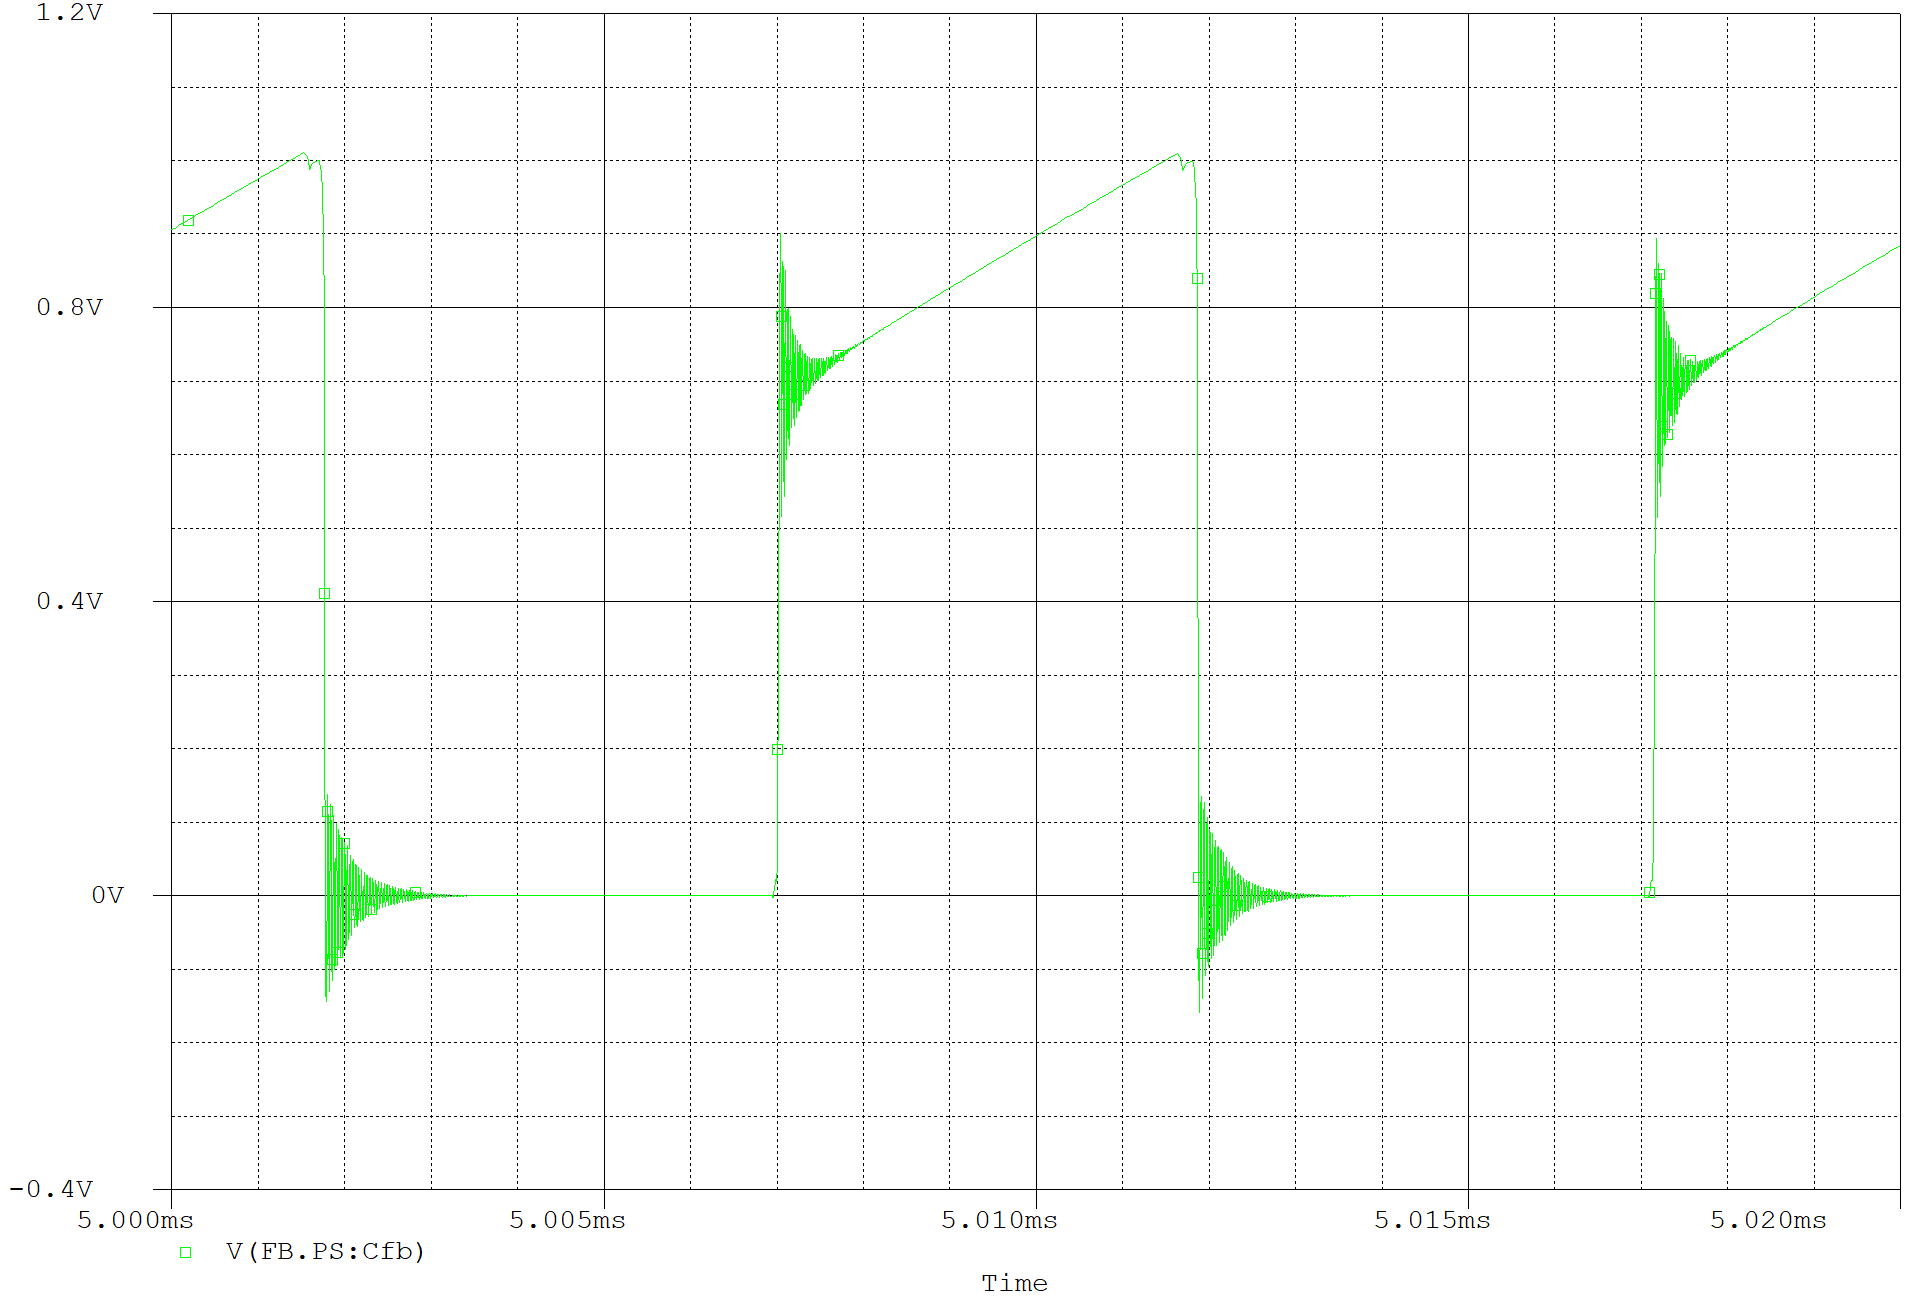
\includegraphics[max width=0.9\linewidth]{/tex/2iteration/billeder/Simulering_PWM_current_sense_U.png}
	\caption{Simulering af current-sense signal før filtrering}
	\label{fig:Simulering_PWM_current_sense_U}
\end{figure}

\begin{figure}[H]
	\center
	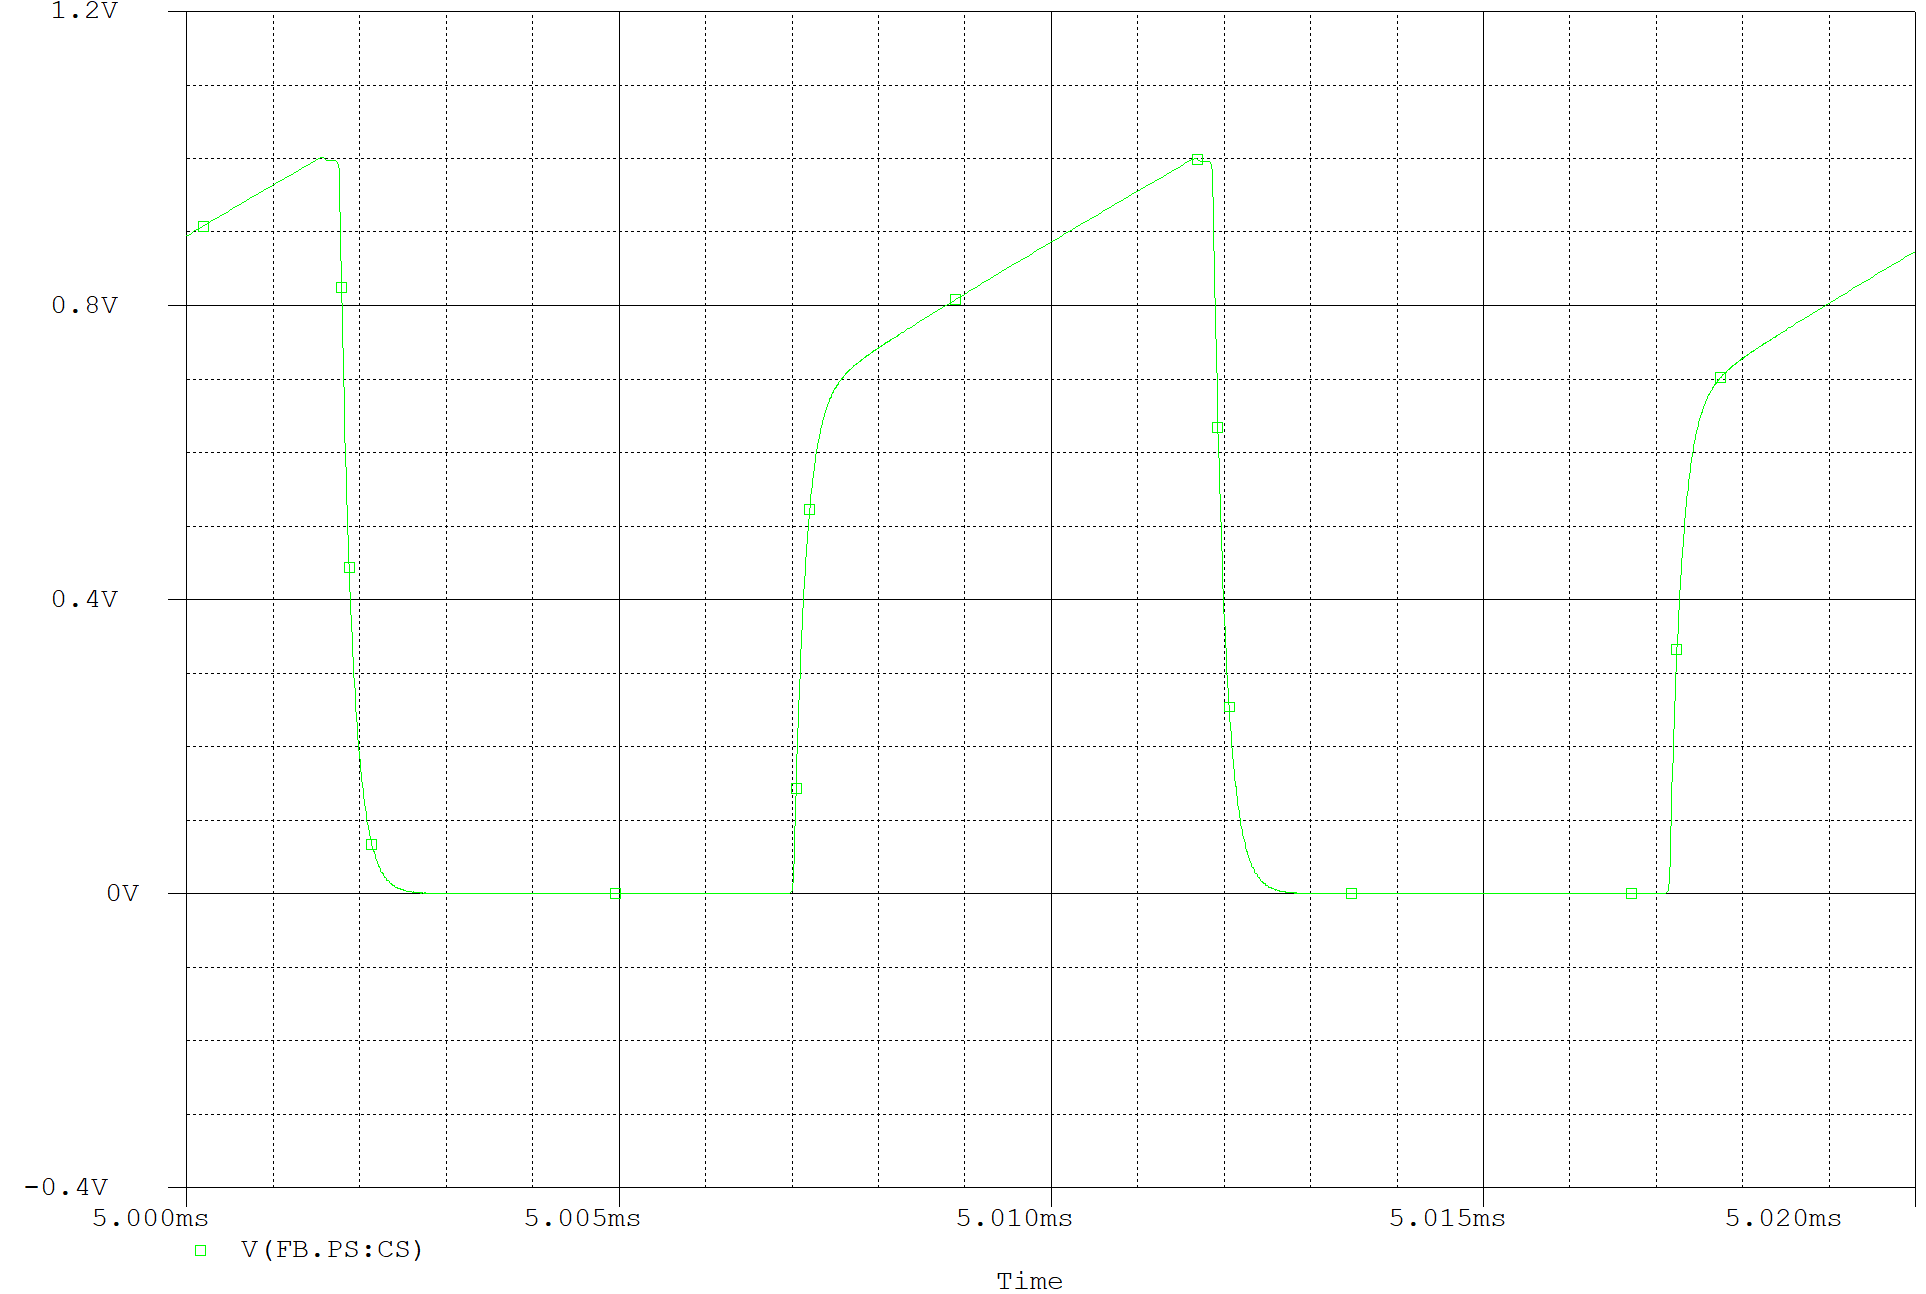
\includegraphics[max width=0.9\linewidth]{/tex/2iteration/billeder/Simulering_PWM_current_sense_M.png}
	\caption{Simulering af current-sense signal efter filtrering}
	\label{fig:Simulering_PWM_current_sense_M}
\end{figure}


